As demonstrated above, some object categories (i.e. animal, person, and vehicle) tend to be more memorable than others. However, not all objects in the same category are equally memorable. The examples in Figure \ref{fig:obLabelQual} show the most memorable, medium memorable, and least memorable objects for each category. Across classes, non-memorable objects tend to be those that are occluded and obstructed by other objects. What other category-related factors could influence the memorability of objects? Among the possible factors, we explore how category-specific object memorability is influenced by \textbf{(i)} the number of objects in an image and \textbf{(ii)} the presence of other object categories. \B{stick to using category instead of class throughout the paper.}

\begin{figure*}[!htb]
\centering
\subfigure{\centering 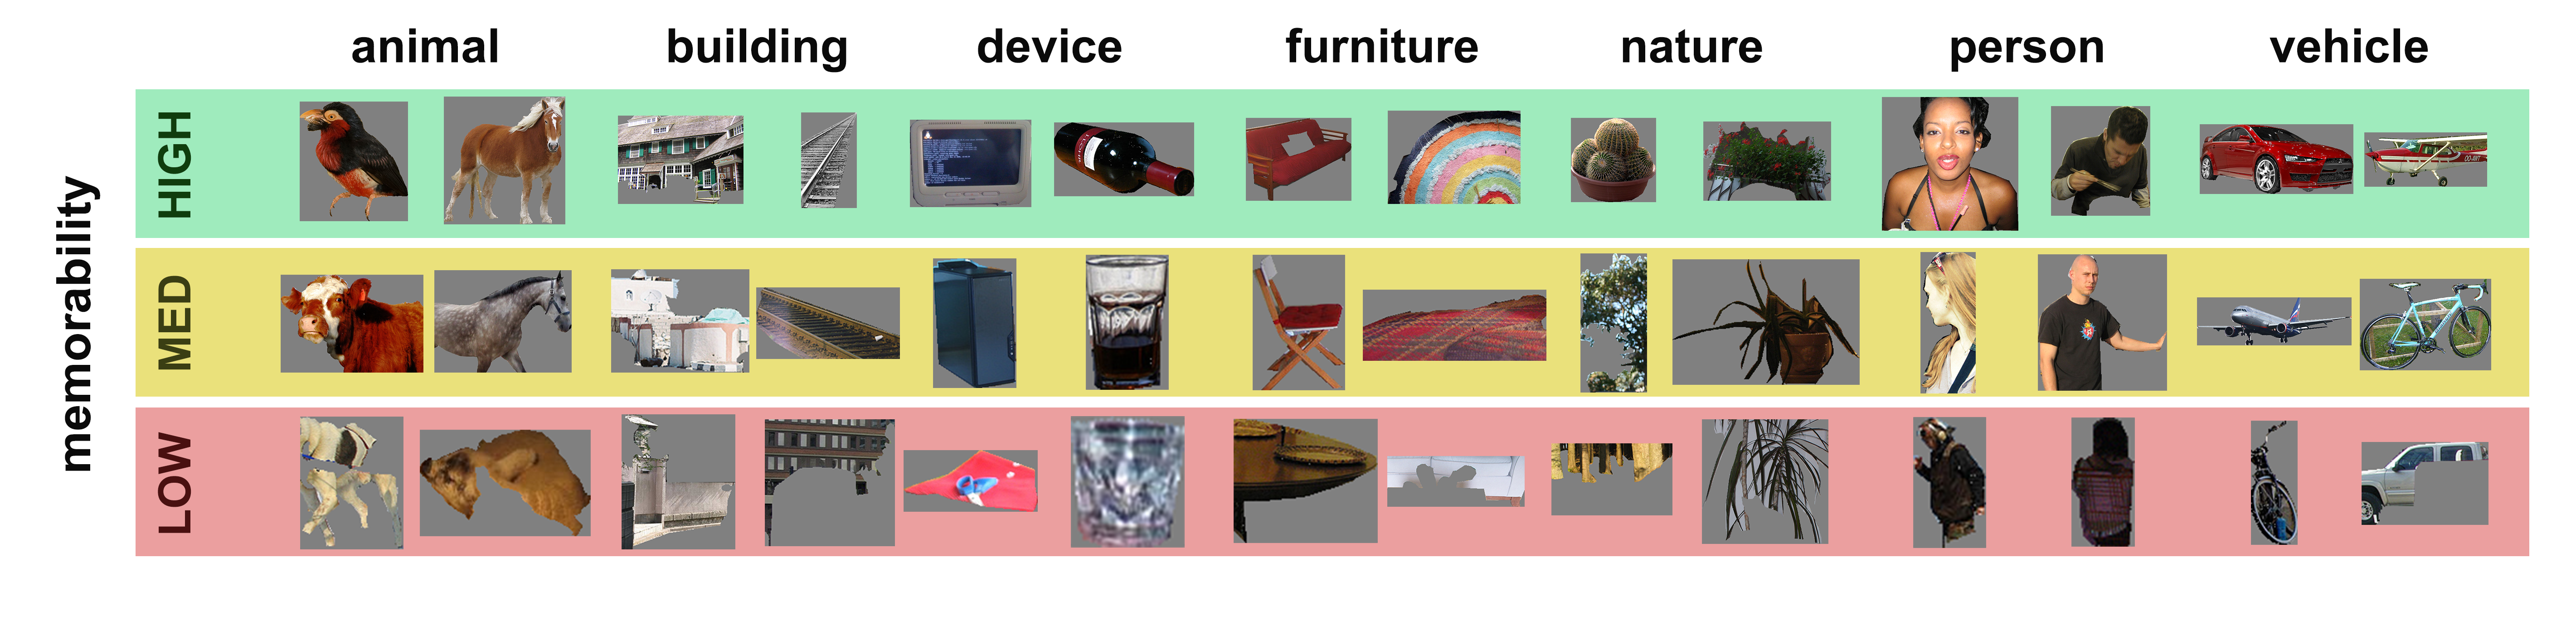
\includegraphics[width=1\textwidth]{figures/results/obLabel/qual_cat_v2.png}}
\vspace{-5mm}\caption{\footnotesize\textbf{Memorability of object categories.} A sample of the most memorable, average memorable and least memorable objects from each of the $7$ object categories in our dataset.}\label{fig:obLabelQual}
\end{figure*}

\noindent\textbf{Number of objects:} %We first examined how the memorability of each object class is affected by the number of objects inside an image.
Figure \ref{fig:obLabelChange} shows the change in average memorability for the different categories when the minimum number of objects within an image is increased. Results indicate that the number of objects present in an image is an important factor in determining memorability. For example, as the number of objects in an image increases, the memorability of animals and vehicles decreases sharply, most likely as a result of competition for attention. Interestingly, the memorability of the person category does not change significantly when an increasing number of objects exist in the image. This suggests that people are not only one of the most memorable object categories, but that their memorability is the least sensitive to the presence of object clutter in an image. This may be because a single person steals most of the viewer's attention in an image, but how is this behavior characterized in the presence of other multiple people in the same image? To answer this, we turn to the question of interclass memorability next.

\begin{figure}[t]
\centering
\subfigure{\centering \includegraphics[width=0.45\textwidth]{figures/results/obLabel/memScore_change2.png}}
\vspace{-5mm}\caption{\footnotesize\textbf{Object number influences category-specific memorability.} For each category, a curve is plotted that shows the change in average memorability with an increase in the number of objects. The memorability of objects belonging to categories like animals and vehicles goes down significantly with an increase in object number.}\label{fig:obLabelChange}
\end{figure}

\begin{figure}[b]
\centering
\subfigure{\centering \includegraphics[width=0.5\textwidth]{figures/results/obLabel/confusionMatrix.png}}
\vspace{-5mm}\caption{\footnotesize\textbf{Inter-class object memorability relationship.} Figure shows the effect that the presence of a distractor category has on each category treated as a reference. }\label{fig:obLabelPair}
\end{figure}

\noindent\textbf{Inter-class memorability:} How much is the memorability of a particular object category affected when it co-occurs with another object category (or another instance of the same category)? To quantify the effect of one category on another, we consider each pairwise combination of categories and gather all images that contain at least one object from both categories. By taking one category as the \emph{reference} and the other as the \emph{distractor}, we compute the average memorability score $m_{R|D}$ of the reference in the  images common to the reference and distractor. To isolate the effect of the distractor, we compute the memorability difference $\Delta m=(m_{R|D}-m_R)$, where $m_R$ is the memorability score of the reference in all images where it exists. Figure \ref{fig:obLabelPair} shows $\Delta m$ for all possible reference and distractor pairs. It is clear that  $\Delta m$ for low-memorability categories (i.e. nature, furniture, device, and building) are not significantly affected by the presence of other categories. %Instead, their memorability tends to remain low across all contexts.


\begin{figure}[!htb]
\centering
\subfigure{\centering \includegraphics[height = 1.1 cm]{figures/results/obLabel/inter-class/14.jpg}}
\subfigure{\centering \includegraphics[height = 1.1 cm]{figures/results/obLabel/inter-class/85.jpg}}
\subfigure{\centering \includegraphics[height = 1.1 cm]{figures/results/obLabel/inter-class/10.jpg}}
\subfigure{\centering \includegraphics[height = 1.1 cm]{figures/results/obLabel/inter-class/128.jpg}}
\subfigure{\centering \includegraphics[height = 1.1 cm]{figures/results/obLabel/inter-class/102.jpg}}
\subfigure{\centering \includegraphics[height = 1.1 cm]{figures/results/obLabel/inter-class/129.jpg}}\\
\vspace{-2mm}
\subfigure{\centering \includegraphics[height = 1.1 cm]{figures/results/obLabel/inter-class/14.png}}
\subfigure{\centering \includegraphics[height = 1.1 cm]{figures/results/obLabel/inter-class/85.png}}
\subfigure{\centering \includegraphics[height = 1.1 cm]{figures/results/obLabel/inter-class/10.png}}
\subfigure{\centering \includegraphics[height = 1.1 cm]{figures/results/obLabel/inter-class/128.png}}
\subfigure{\centering \includegraphics[height = 1.1 cm]{figures/results/obLabel/inter-class/102.png}}
\subfigure{\centering \includegraphics[height = 1.1 cm]{figures/results/obLabel/inter-class/129.png}}
\vspace{-5mm}\caption{\footnotesize\textbf{Memorability of person category in presence of other categories.} Top row: example images where a person is present along with other competing categories. Bottom row: Ground truth object memorability maps. In the presence of buildings, the memorability of person can drop due to the contrasting sizes. In the presence of a vehicle, or an animal, the person usually is more memorable to humans. }\label{fig:qualInterClass}
\end{figure}

On the other hand, the memorability of the animal category maintains its high score in the presence of other categories, except vehicles, people, and itself, where it decreases substantially. The memorability of people tends to be unaffected by the presence of most other categories including itself. However, it decreases in the presence of vehicles and buildings. This could be due to the fact that people in images containing vehicles or buildings are usually zoomed out and are usually smaller in size (refer to Figure \ref{fig:qualInterClass} for  examples). The memorability of the vehicle category is strongly affected by the presence of other object categories. In particular, it drops significantly in the presence of another vehicle, people, and animals.

In summary, when an animal, vehicle or a person co-occur in the same image, the memorability of all three categories usually decreases. However, this pattern of change in memorability is category-specific in general. For example, when a vehicle and animal are present in the same image, the animal is generally more memorable, even though both their memorability scores drop significantly. When a vehicle or an animal co-occurs with a person, the person is generally more memorable (also shown in Figure \ref{fig:qualInterClass}).





